% Keep Wiley's supplied class and support files in their own directory while
% making that directory available to package lookups performed by USG.cls.
\makeatletter
\def\input@path{{latex/wiley/}}
\makeatother
\documentclass[ASNA]{latex/wiley/USG}

% Retain the supplied class for the manuscript body, but use a deliberately
% plain author-manuscript front matter with no journal branding or publication
% metadata. The additional packages support manuscript tables, supplementary
% landscape pages, and the blue/red revision markup.
\usepackage{anyfontsize}
\usepackage{fontspec}
\setmainfont{STIX-Regular.otf}[
  Path=latex/wiley/Fonts/Stix/,
  BoldFont=STIX-Bold.otf,
  ItalicFont=STIX-Italic.otf,
  BoldItalicFont=STIX-BoldItalic.otf
]
\usepackage{colortbl}
\usepackage{xcolor}
\usepackage{longtable}
\newcounter{none}
\renewcommand{\thenone}{}
\usepackage{pdflscape}
\usepackage{caption}
\usepackage{hanging}
\usepackage[section]{placeins}

\graphicspath{{FlowMOP_submission_media/}{figs_data/}}

\definecolor{revisionblue}{HTML}{0066CC}
\definecolor{revisionred}{HTML}{C00000}
\providecommand{\tightlist}{\setlength{\itemsep}{0pt}\setlength{\parskip}{0pt}}
\providecommand{\pandocbounded}[1]{#1}
\providecommand{\passthrough}[1]{#1}


\begin{document}

\pagestyle{plain}
\floatpagestyle{plain}
\rotfloatpagestyle{plain}
\setlength{\parindent}{0pt}
\setlength{\parskip}{\baselineskip}
\raggedbottom

% \aff prints an affiliation number. The Supporting Information has no
% affiliation list, so there it prints nothing.
\newcommand{\aff}[1]{}
\begin{center}
{\LARGE\bfseries Supporting Information\par}
\vspace{1em}
{\large\bfseries FlowMOP: An Automated Flow Cytometry Time, Debris, and
Doublet Removal Tool\par}
\vspace{1em}
{\normalsize
Tony Xu\aff{1},
Nadia A. Roberts\aff{1},
Felix Marsh-Wakefield\aff{2,3},
Rebecca A. Jaeger\aff{1},
Sarah Croft\aff{1},
Abhimanu Pandey\aff{1},
Dalton Leibold\aff{4},
Angela L. Ferguson\aff{2,3},
Lily Rodgers\aff{2,3},
Umaimainthan Palendira\aff{3},
Geoffrey W. McCaughan\aff{2,5,6},
Ben Quah\aff{7},
Robin Vlieger\aff{8}, and
Anne Brüstle\aff{1,*}\par}
\end{center}




\FloatBarrier

\section{Supplementary data}\label{supplementary-data}

\begin{figure}[p]
\centering
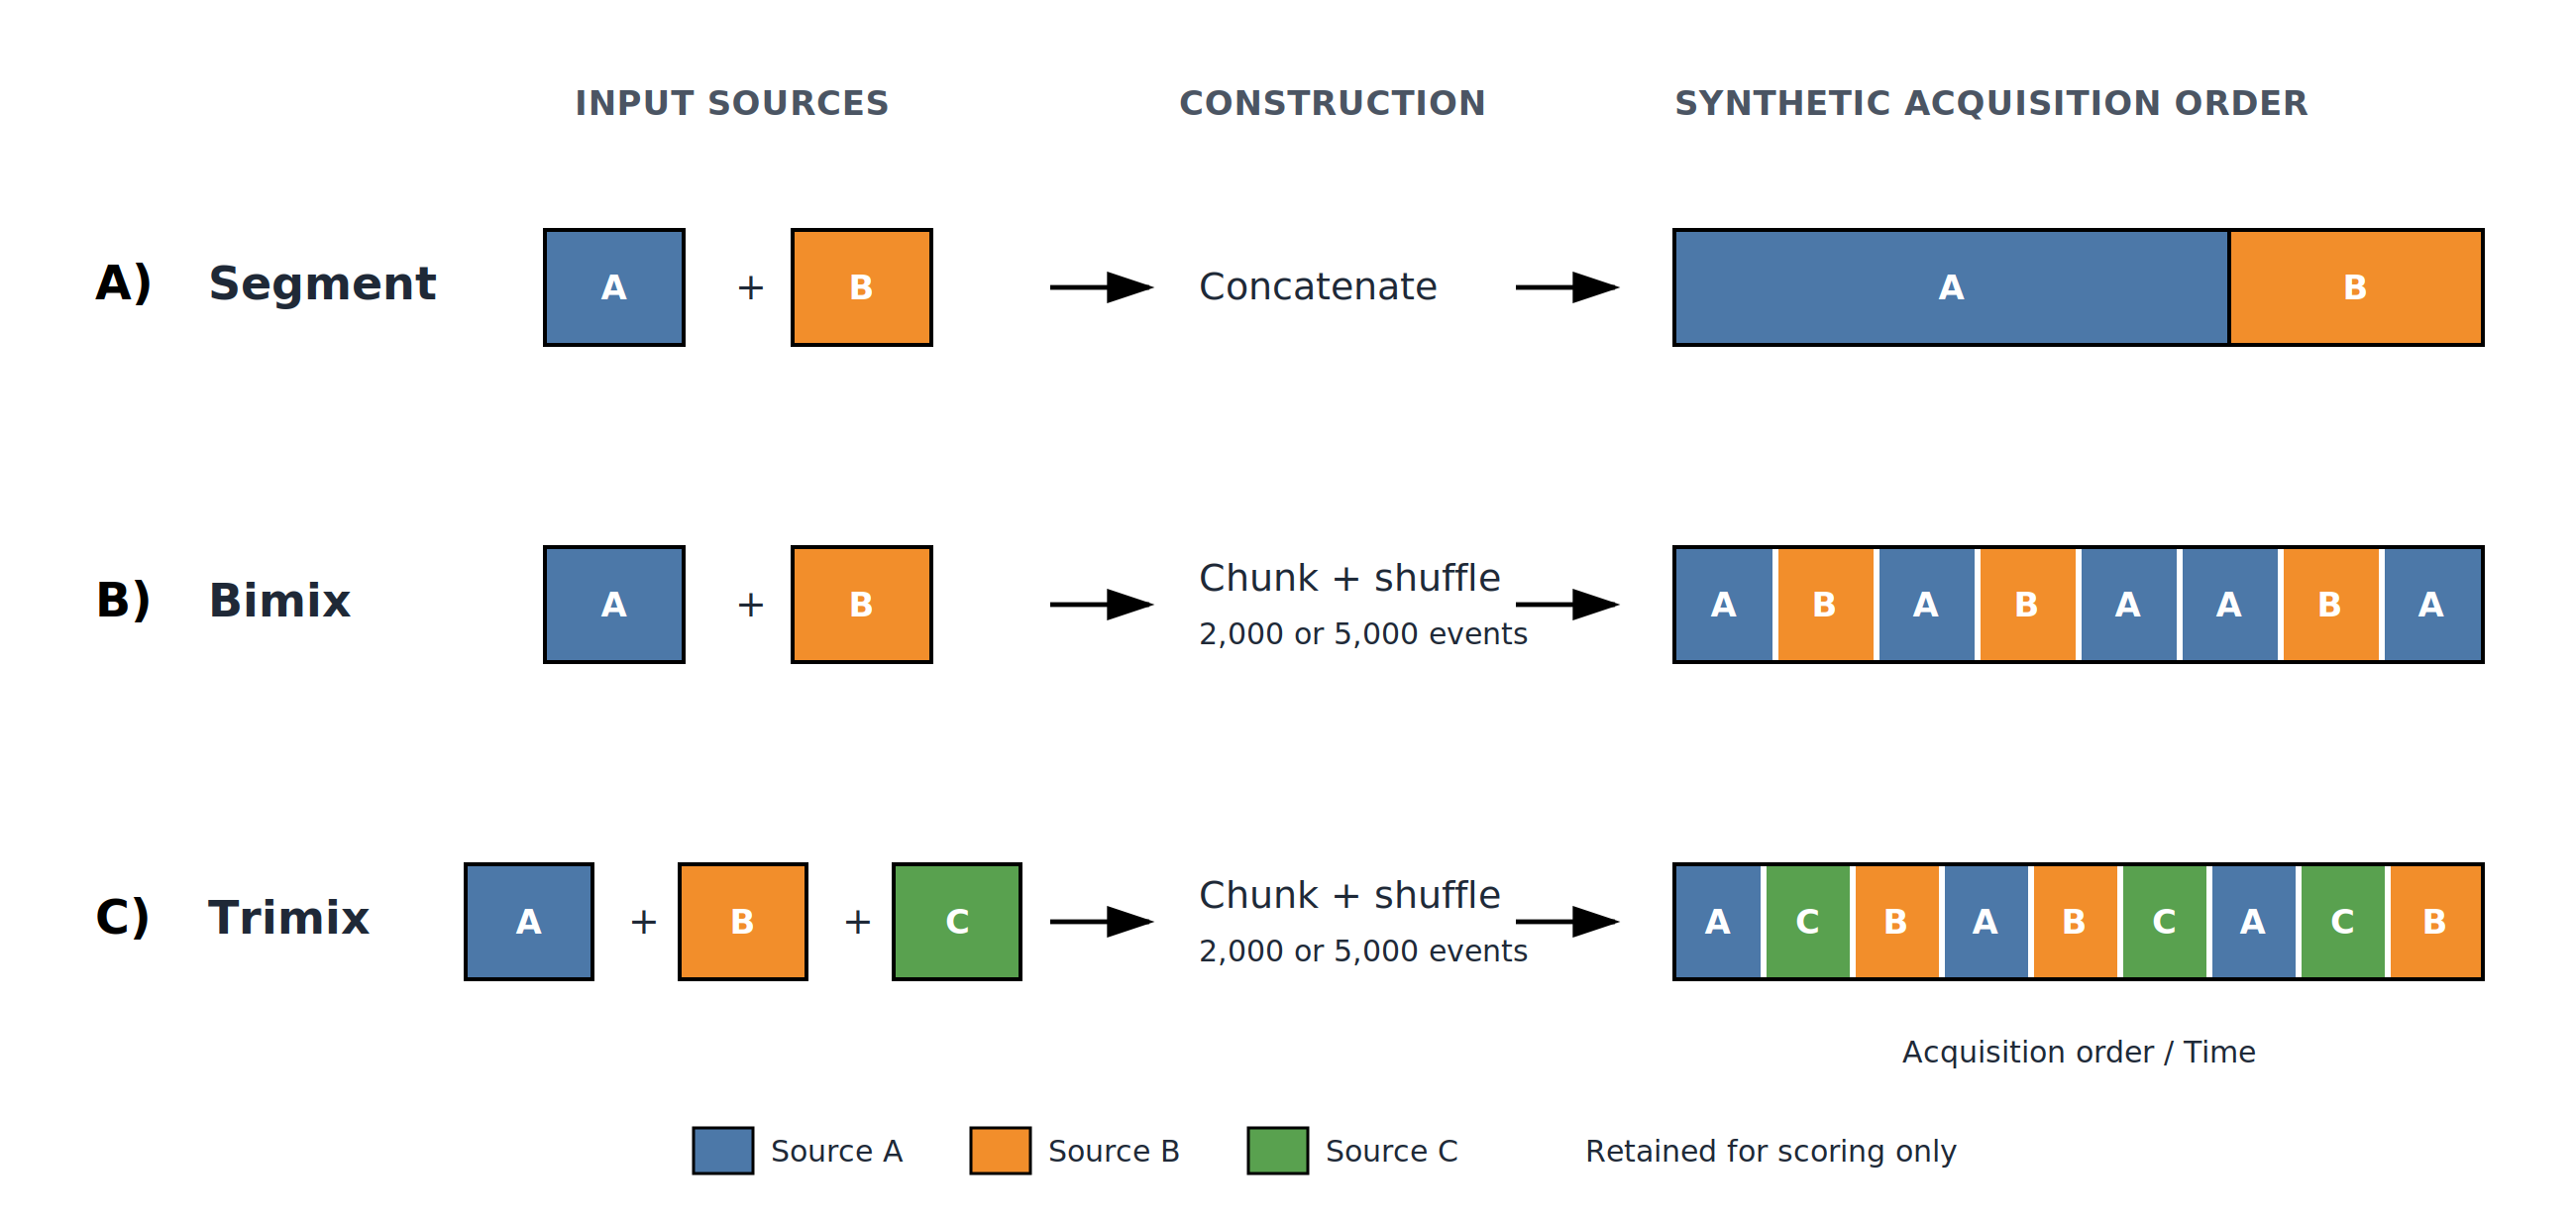
\includegraphics[width=\linewidth,height=0.82\textheight,keepaspectratio]{figs_data/synthetic_time_design_schematic.png}
\begingroup
\renewcommand{\thefigure}{S1}
\caption{Construction of Segment, Bimix, and Trimix synthetic time samples. No flow-rate disturbance was introduced.}
\endgroup
\end{figure}

\begin{figure}[p]
\centering
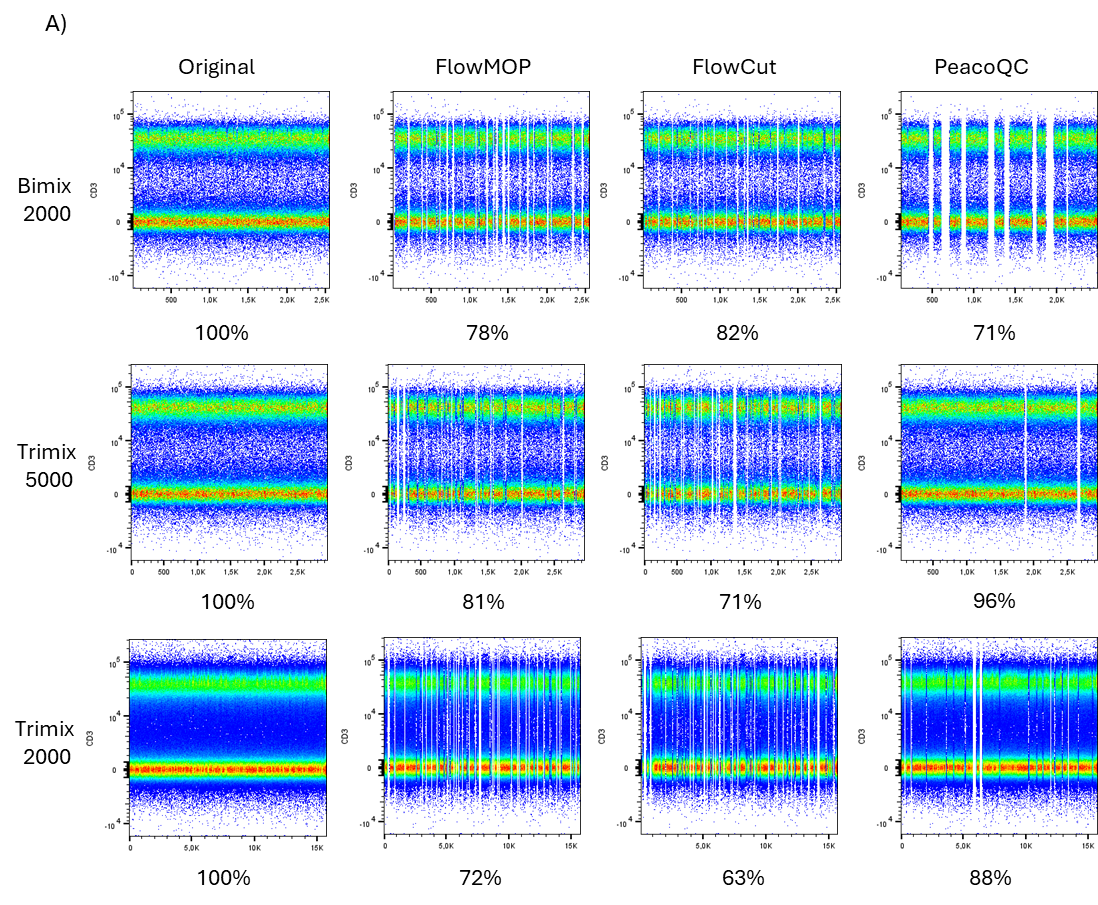
\includegraphics[width=\linewidth,height=0.82\textheight,keepaspectratio]{FlowMOP_submission_media/image8.png}
\begingroup
\renewcommand{\thefigure}{S2}
\caption{Representative CD3-versus-Time plots for Bimix samples with 2,000-event bins and Trimix samples with 2,000- and 5,000-event bins, showing the original inputs and outputs after cleaning with FlowMOP, FlowCut, and PeacoQC. Percentages below each figure represent the retained proportion of cells relative to the original representative synthetic sample.}
\endgroup
\end{figure}

\begingroup
\small
\setlength{\tabcolsep}{4pt}
\renewcommand{\arraystretch}{1.14}

\captionsetup{type=table}
\begingroup
\renewcommand{\thetable}{S1}
\captionof{table}{\textbf{Dataset Compositions}}
\endgroup

{\def\LTcaptype{none} % do not increment counter
\begin{longtable}[]{@{}
  >{\raggedright\arraybackslash}p{(\linewidth - 8\tabcolsep) * \real{0.1920}}
  >{\raggedright\arraybackslash}p{(\linewidth - 8\tabcolsep) * \real{0.1920}}
  >{\raggedright\arraybackslash}p{(\linewidth - 8\tabcolsep) * \real{0.1920}}
  >{\raggedright\arraybackslash}p{(\linewidth - 8\tabcolsep) * \real{0.1920}}
  >{\raggedright\arraybackslash}p{(\linewidth - 8\tabcolsep) * \real{0.1920}}@{}}
\toprule\noalign{}
\begin{minipage}[b]{\linewidth}\raggedright
Dataset Name
\end{minipage} & \begin{minipage}[b]{\linewidth}\raggedright
Synthetic Time-Gating Dataset
\end{minipage} & \begin{minipage}[b]{\linewidth}\raggedright
Synthetic Debris-Gating Dataset
\end{minipage} & \begin{minipage}[b]{\linewidth}\raggedright
Synthetic Doublet-Gating Dataset
\end{minipage} & \begin{minipage}[b]{\linewidth}\raggedright
Human Liver
\end{minipage} \\
\midrule\noalign{}
\endhead
\bottomrule\noalign{}
\endlastfoot
Samples (given per benchmarker) & 6, 2 each at 0.5, 1, 3 cell
concentrations, 3 datasets & 4, combined into 3 benchmarking samples &
4, combined into 3 benchmarking samples & 3 \\
Tissue Type & Peripheral blood mononuclear cells & Spleen & Spleen &
Liver tissue \\
Organism & Human & Mouse & Mouse & Human \\
Collection Location & Canberra, ACT, Australia & Canberra, ACT,
Australia & Canberra, ACT, Australia & Sydney, NSW, Australia \\
\end{longtable}
}

\endgroup

\begingroup
\small
\setlength{\tabcolsep}{4pt}
\renewcommand{\arraystretch}{1.14}

{\def\LTcaptype{none} % do not increment counter
\begin{longtable}[]{@{}
  >{\raggedright\arraybackslash}p{(\linewidth - 8\tabcolsep) * \real{0.1920}}
  >{\raggedright\arraybackslash}p{(\linewidth - 8\tabcolsep) * \real{0.1920}}
  >{\raggedright\arraybackslash}p{(\linewidth - 8\tabcolsep) * \real{0.1920}}
  >{\raggedright\arraybackslash}p{(\linewidth - 8\tabcolsep) * \real{0.1920}}
  >{\raggedright\arraybackslash}p{(\linewidth - 8\tabcolsep) * \real{0.1920}}@{}}
\toprule\noalign{}
\begin{minipage}[b]{\linewidth}\raggedright
Mouse Dorsal Root Ganglion
\end{minipage} & \begin{minipage}[b]{\linewidth}\raggedright
Mouse Skin
\end{minipage} & \begin{minipage}[b]{\linewidth}\raggedright
Mouse Small Intestine
\end{minipage} & \begin{minipage}[b]{\linewidth}\raggedright
Mouse Colon
\end{minipage} & \begin{minipage}[b]{\linewidth}\raggedright
Mouse Brain
\end{minipage} \\
\midrule\noalign{}
\endhead
\bottomrule\noalign{}
\endlastfoot
3 & 3 & 3 & 3 & 4 \\
Dorsal root ganglia & Skin & Distal small intestine & Colon & Brain \\
Mouse & Mouse & Mouse & Mouse & Mouse \\
Canberra, ACT, Australia & Canberra, ACT, Australia & Canberra, ACT,
Australia & Canberra, ACT, Australia & Canberra, ACT, Australia \\
\end{longtable}
}

\endgroup

\begingroup
\small
\setlength{\tabcolsep}{4pt}
\renewcommand{\arraystretch}{1.14}

{\def\LTcaptype{none} % do not increment counter
\begin{longtable}[]{@{}
  >{\raggedright\arraybackslash}p{(\linewidth - 8\tabcolsep) * \real{0.1920}}
  >{\raggedright\arraybackslash}p{(\linewidth - 8\tabcolsep) * \real{0.1920}}
  >{\raggedright\arraybackslash}p{(\linewidth - 8\tabcolsep) * \real{0.1920}}
  >{\raggedright\arraybackslash}p{(\linewidth - 8\tabcolsep) * \real{0.1920}}
  >{\raggedright\arraybackslash}p{(\linewidth - 8\tabcolsep) * \real{0.1920}}@{}}
\toprule\noalign{}
\begin{minipage}[b]{\linewidth}\raggedright
Mouse Central Nervous System
\end{minipage} & \begin{minipage}[b]{\linewidth}\raggedright
Mouse Spleen
\end{minipage} & \begin{minipage}[b]{\linewidth}\raggedright
Mouse Blood
\end{minipage} & \begin{minipage}[b]{\linewidth}\raggedright
Mouse Bone Marrow
\end{minipage} & \begin{minipage}[b]{\linewidth}\raggedright
Human Cultured T cells
\end{minipage} \\
\midrule\noalign{}
\endhead
\bottomrule\noalign{}
\endlastfoot
3 & 7 & 5 & 3 & 5 \\
Spinal cord and brain & Spleen & Peripherally collected blood & Femur
derived bone marrow & Peripherally collected, cultured, and restimulated
T cells \\
Mouse & Mouse & Mouse & Mouse & Human \\
Canberra, ACT, Australia & Canberra, ACT, Australia & Canberra, ACT,
Australia & Canberra, ACT, Australia & Canberra, ACT, Australia \\
\end{longtable}
}

\endgroup

\begingroup
\small
\setlength{\tabcolsep}{4pt}
\renewcommand{\arraystretch}{1.14}

\captionsetup{type=table}
\begingroup
\renewcommand{\thetable}{S2}
\captionof{table}{\textbf{Jeffreys' Scale}}
\endgroup

{\def\LTcaptype{none} % do not increment counter
\begin{longtable}[]{@{}ll@{}}
\toprule\noalign{}
Bayes Factor & Hypothesis descriptor \\
\midrule\noalign{}
\endhead
\bottomrule\noalign{}
\endlastfoot
\textless1 & Null hypothesis supported \\
1-3 & Anecdotal / Weak evidence \\
3-10 & Moderate / Substantial evidence \\
10-30 & Very strong evidence \\
\textgreater30 & Decisive evidence \\
\end{longtable}
}

\endgroup

\clearpage
\begin{landscape}
\begingroup
\scriptsize
\setlength{\tabcolsep}{3pt}
\renewcommand{\arraystretch}{1.12}

\captionsetup{type=table}
\begingroup
\renewcommand{\thetable}{S3}
\captionof{table}{\textbf{Limit-of-detection precleaning in biological-validation inputs}}
\endgroup

Events with passed\_lod values below 0.5 were counted as removed.
FlowMOP removes maximum-FSC-A events only when they exceed 1\% of the
input. This 1\% cutoff is an arbitrary operational safeguard, not an
empirically optimized biological threshold. Activation depends on
acquisition scaling and voltage/gain settings; the observed activation
rates are dataset-specific and should not be generalized across
instruments.

{\def\LTcaptype{none} % do not increment counter
\begin{longtable}[]{@{}
  >{\raggedright\arraybackslash}p{(\linewidth - 10\tabcolsep) * \real{0.1600}}
  >{\raggedleft\arraybackslash}p{(\linewidth - 10\tabcolsep) * \real{0.1600}}
  >{\raggedleft\arraybackslash}p{(\linewidth - 10\tabcolsep) * \real{0.1600}}
  >{\raggedleft\arraybackslash}p{(\linewidth - 10\tabcolsep) * \real{0.1600}}
  >{\raggedleft\arraybackslash}p{(\linewidth - 10\tabcolsep) * \real{0.1600}}
  >{\raggedright\arraybackslash}p{(\linewidth - 10\tabcolsep) * \real{0.1600}}@{}}
\toprule\noalign{}
\begin{minipage}[b]{\linewidth}\raggedright
Dataset
\end{minipage} & \begin{minipage}[b]{\linewidth}\raggedleft
Sample
\end{minipage} & \begin{minipage}[b]{\linewidth}\raggedleft
Input events
\end{minipage} & \begin{minipage}[b]{\linewidth}\raggedleft
Events removed
\end{minipage} & \begin{minipage}[b]{\linewidth}\raggedleft
Events removed (\%)
\end{minipage} & \begin{minipage}[b]{\linewidth}\raggedright
Threshold activated
\end{minipage} \\
\midrule\noalign{}
\endhead
\bottomrule\noalign{}
\endlastfoot
PBMC & 1 & 143,656 & 0 & 0.00 & No \\
PBMC & 2 & 426,248 & 0 & 0.00 & No \\
PBMC & 3 & 463,512 & 0 & 0.00 & No \\
PBMC & 4 & 258,952 & 0 & 0.00 & No \\
PBMC & 5 & 140,936 & 0 & 0.00 & No \\
PBMC & 6 & 161,704 & 0 & 0.00 & No \\
PBMC & 7 & 242,344 & 0 & 0.00 & No \\
PBMC & 8 & 188,936 & 0 & 0.00 & No \\
Tumour & 1 & 287,752 & 6,863 & 2.39 & Yes \\
Tumour & 2 & 145,520 & 3,472 & 2.39 & Yes \\
Tumour & 3 & 301,872 & 9,206 & 3.05 & Yes \\
\end{longtable}
}

\endgroup
\end{landscape}
\clearpage

\begingroup
\small
\setlength{\tabcolsep}{4pt}
\renewcommand{\arraystretch}{1.14}

\captionsetup{type=table}
\begingroup
\renewcommand{\thetable}{S4}
\captionof{table}{\textbf{Full-dataset FlowMOP MAD-smoothing analysis}}
\endgroup

{\def\LTcaptype{none} % do not increment counter
\begin{longtable}[]{@{}lrrr@{}}
\toprule\noalign{}
Short, long smoothing factors & Sensitivity & Specificity & Balanced
mean \\
\midrule\noalign{}
\endhead
\bottomrule\noalign{}
\endlastfoot
0,0 (no-smoothing control) & 0.8021 & \textbf{0.7081} &
\textbf{0.75506} \\
\textbf{0.01,0.05 (current default)} & 0.8212 & 0.6811 &
\textbf{0.75114} \\
0.02,0.05 & 0.8228 & 0.6794 & 0.75108 \\
0.01,0.02 & 0.8112 & 0.6885 & 0.74986 \\
0.02,0.09 & \textbf{0.8276} & 0.6709 & 0.74923 \\
0.01,0.09 & 0.8257 & 0.6707 & 0.74823 \\
0.05,0.09 & 0.8188 & 0.6676 & 0.74317 \\
0.02,0.20 & 0.8248 & 0.6479 & 0.73632 \\
0.05,0.20 & 0.8197 & 0.6520 & 0.73586 \\
0.01,0.20 & 0.8231 & 0.6477 & 0.73540 \\
0.10,0.20 & 0.8138 & 0.6415 & 0.72769 \\
0.05,0.34 & 0.8194 & 0.6344 & 0.72686 \\
0.02,0.34 & 0.8199 & 0.6286 & 0.72424 \\
0.10,0.34 & 0.8134 & 0.6250 & 0.71921 \\
0.10,0.50 & 0.8139 & 0.6229 & 0.71842 \\
0.10,0.90 (former default) & 0.8139 & 0.6226 & 0.71827 \\
0.10,1.00 & 0.8139 & 0.6226 & 0.71827 \\
0.20,0.90 & 0.8007 & 0.6142 & 0.70747 \\
0.40,0.90 & 0.7812 & 0.6140 & 0.69756 \\
\end{longtable}
}

\endgroup

Values are equally weighted macro-averages across the six Figure 2
benchmark groups (173 primary inputs; six tied-composition inputs
excluded). The balanced mean is the arithmetic mean of sensitivity and
specificity. Bold indicates the highest value overall and the highest
balanced mean among smoothed settings.

\begin{figure}[p]
\centering
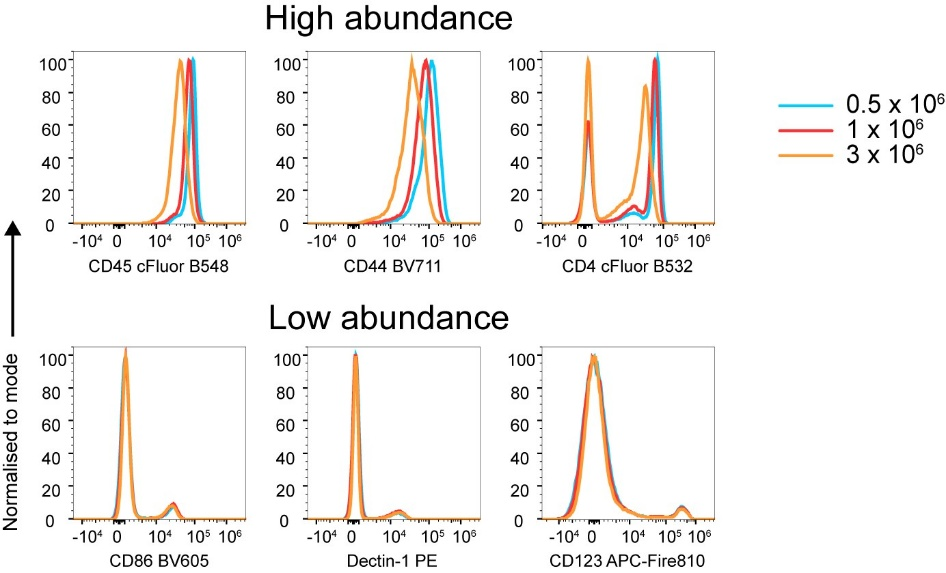
\includegraphics[width=\linewidth,height=0.82\textheight,keepaspectratio]{FlowMOP_submission_media/image9.jpeg}
\begingroup
\renewcommand{\thefigure}{S3}
\caption{Fluorescence variation as a function of cell concentration.}
\endgroup
\end{figure}

\begin{figure}[p]
\centering
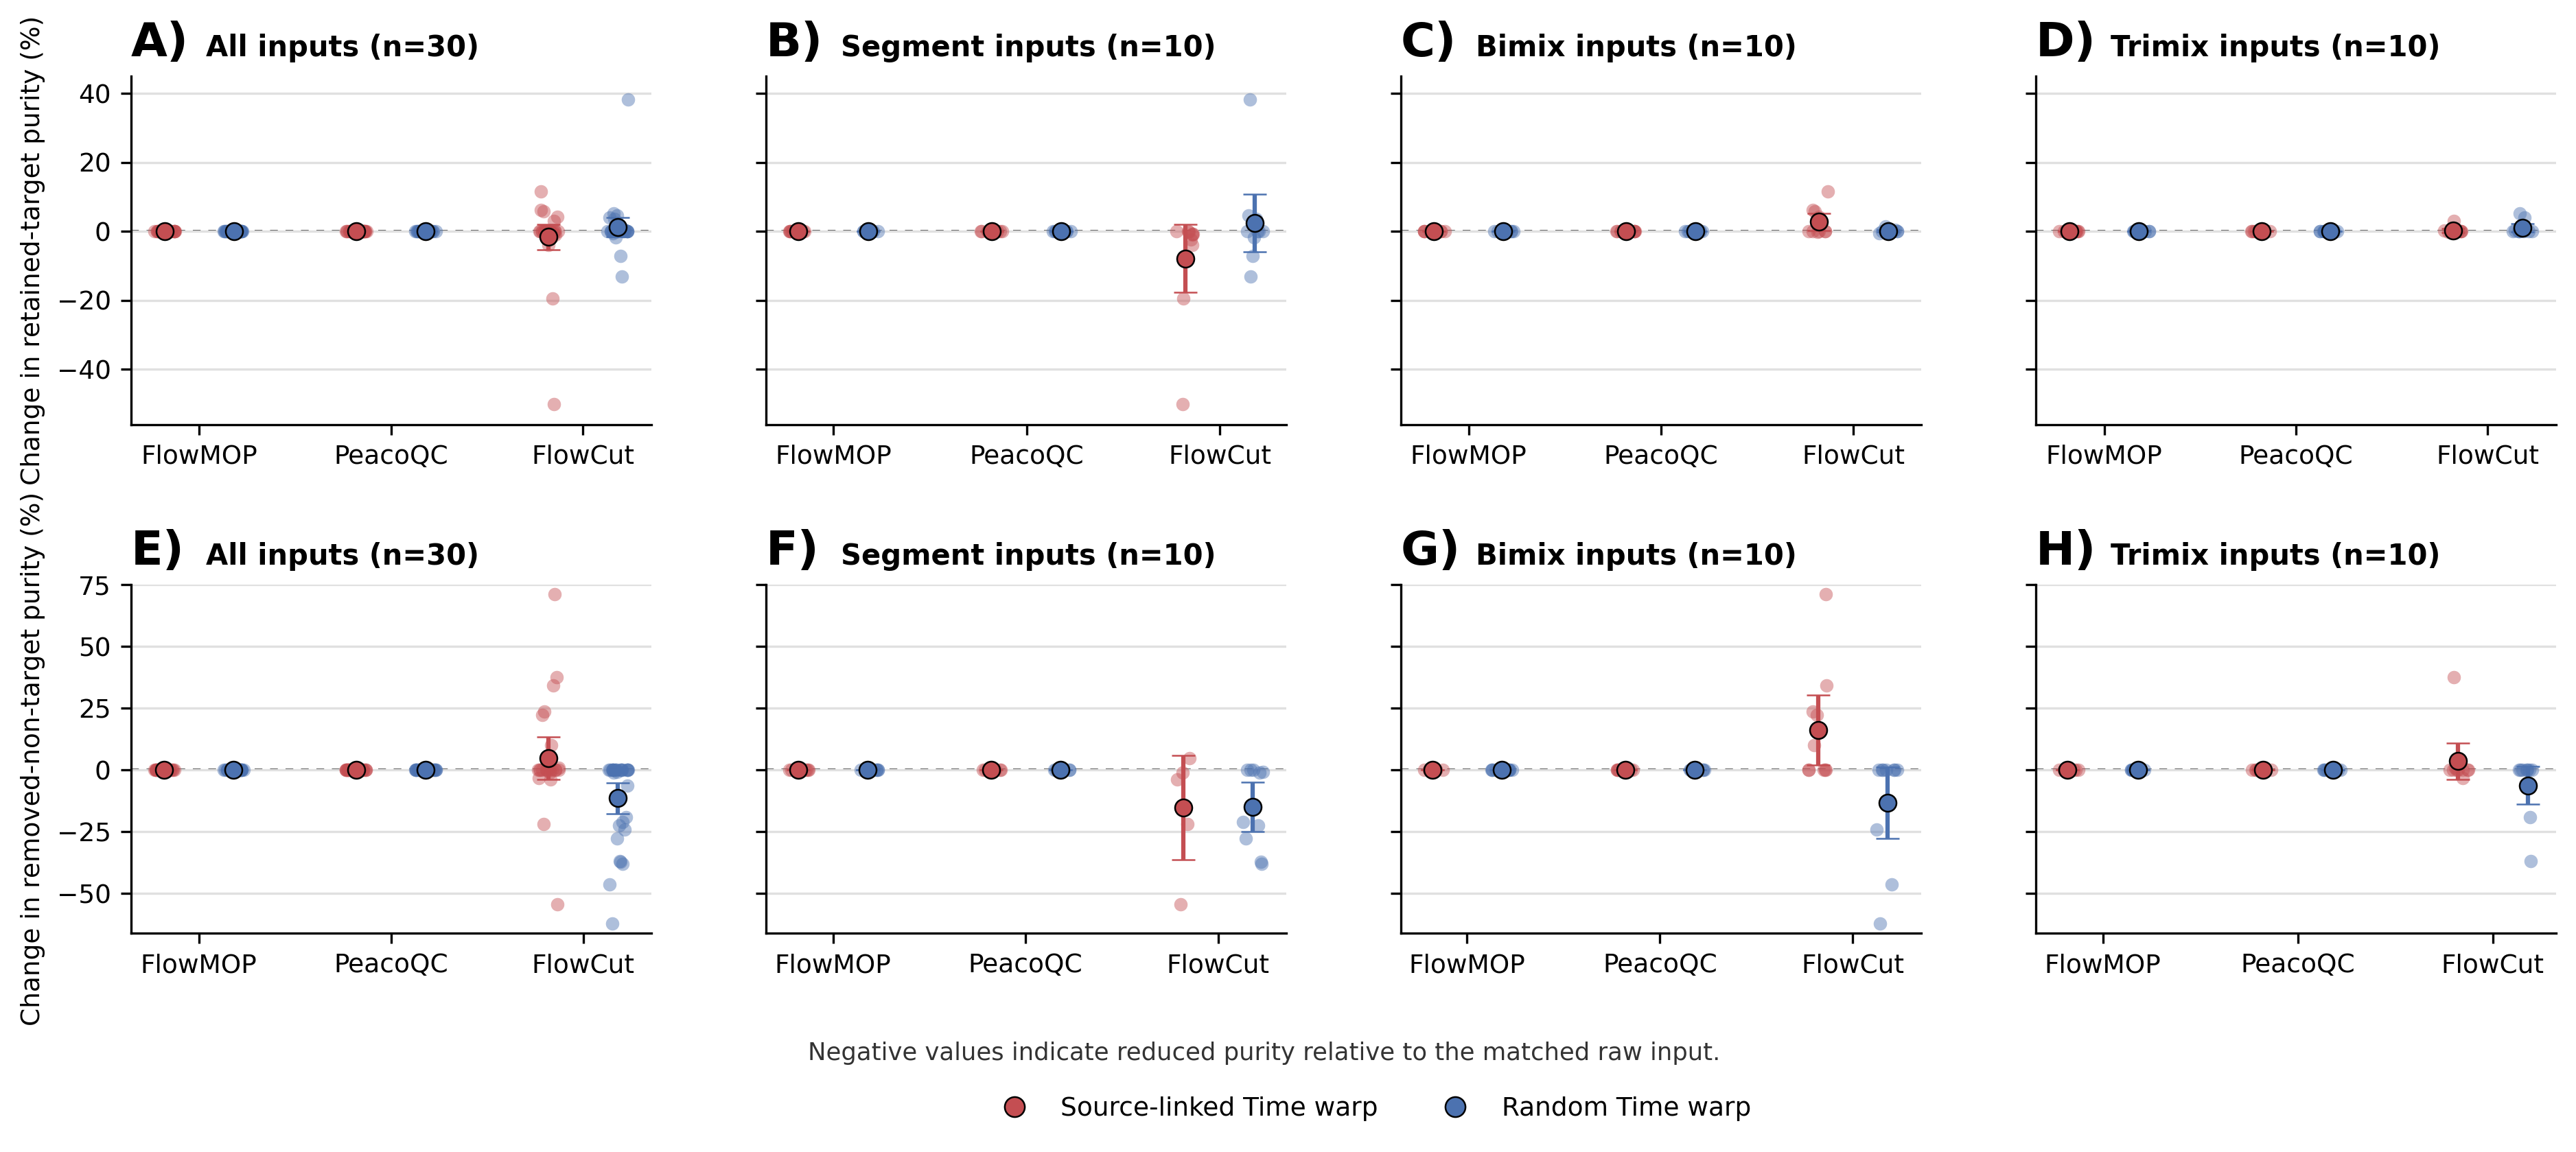
\includegraphics[width=\linewidth,height=0.82\textheight,keepaspectratio]{figs_data/revision_timewarp_mechanism.png}
\begingroup
\renewcommand{\thefigure}{S4}
\caption{Time-only acquisition-rate perturbations reveal FlowCut sensitivity to local Time density. Points show raw-matched changes in sensitivity (A-D) and specificity (E-H), with large points and intervals showing the mean and 95\% confidence interval. Negative values indicate reduced performance relative to the raw control. Columns show all inputs together and the Segment, Bimix, and Trimix subsets separately. FlowMOP and PeacoQC remain unchanged under both source-linked and random Time warping. In contrast, FlowCut\textquotesingle s sensitivity and specificity shift after Time-only perturbation, with the clearest specificity loss in random Time-warped inputs and the strongest source-linked sensitivity loss in Segment inputs, where acquisition-rate structure aligns with source composition.}
\endgroup
\end{figure}

\subsection{Supplementary expert preference
evaluation}\label{supplementary-expert-preference-evaluation}

\subsubsection{Supplementary methods}\label{supplementary-methods}

The expert-ranking analysis was used to summarize relative preferences
among gates generated by FlowMOP, comparator algorithms, and human
operators; it was not treated as an absolute measure of gating adequacy
{[}S1{]}.

Rankings were modelled using a Plackett--Luce model with latent method
abilities; identifiability was enforced by fixing a reference ability to
zero. Independent Normal priors were placed on non-reference abilities.
Posterior inference was performed with an affine-invariant ensemble
Markov Chain Monte Carlo sampler (emcee; 32 walkers, 5,000 iterations;
1,000 burn-in), and posterior medians with 95\% credible intervals were
reported. Directional hypotheses (superiority/inferiority) were
evaluated by computing P = Pr(H1 \textbar{} data) and converting to a
Bayes factor BF$_{10}$ = p/(1 -- p) under equal prior odds, interpreted
using Jeffreys' scale and reported as BF, P (Bayes factor, posterior
probability of the alternative hypothesis) (Table S2).

For each Plackett--Luce fit, the ensemble sampler's mean acceptance
fraction and an integrated-autocorrelation-time-based effective sample
size were monitored (both as implemented in emcee) to assess MCMC
convergence. Across all analyses, mean acceptance fractions ranged from
0.520 to 0.60, and effective sample sizes ranged from 128,003 to
134,042.

Posterior predictive checks compared observed pairwise win counts with
those implied by posterior draws under a Bradley--Terry formulation,
using a chi-square-type discrepancy averaged over method pairs. The
maximum average χ² per comparison was 0.56, indicating good agreement
between the model and the observed rankings.

Computations were implemented in Python with numerically stable
log-likelihoods.

\subsubsection{Supplementary results}\label{supplementary-results}

FlowMOP outputs were compared with expert-provided gates using a
forced-ranking preference task across nine biological datasets. These
rankings measure relative expert preference and should not be
interpreted as an absolute measure of gating adequacy. The resulting
time, debris, and doublet gates were ranked by an expert familiar with
that sample type. FlowCut and PeacoQC were also included in the
time-gating comparison. Rank 1 indicates greatest preference.

\begin{figure}[p]
\centering
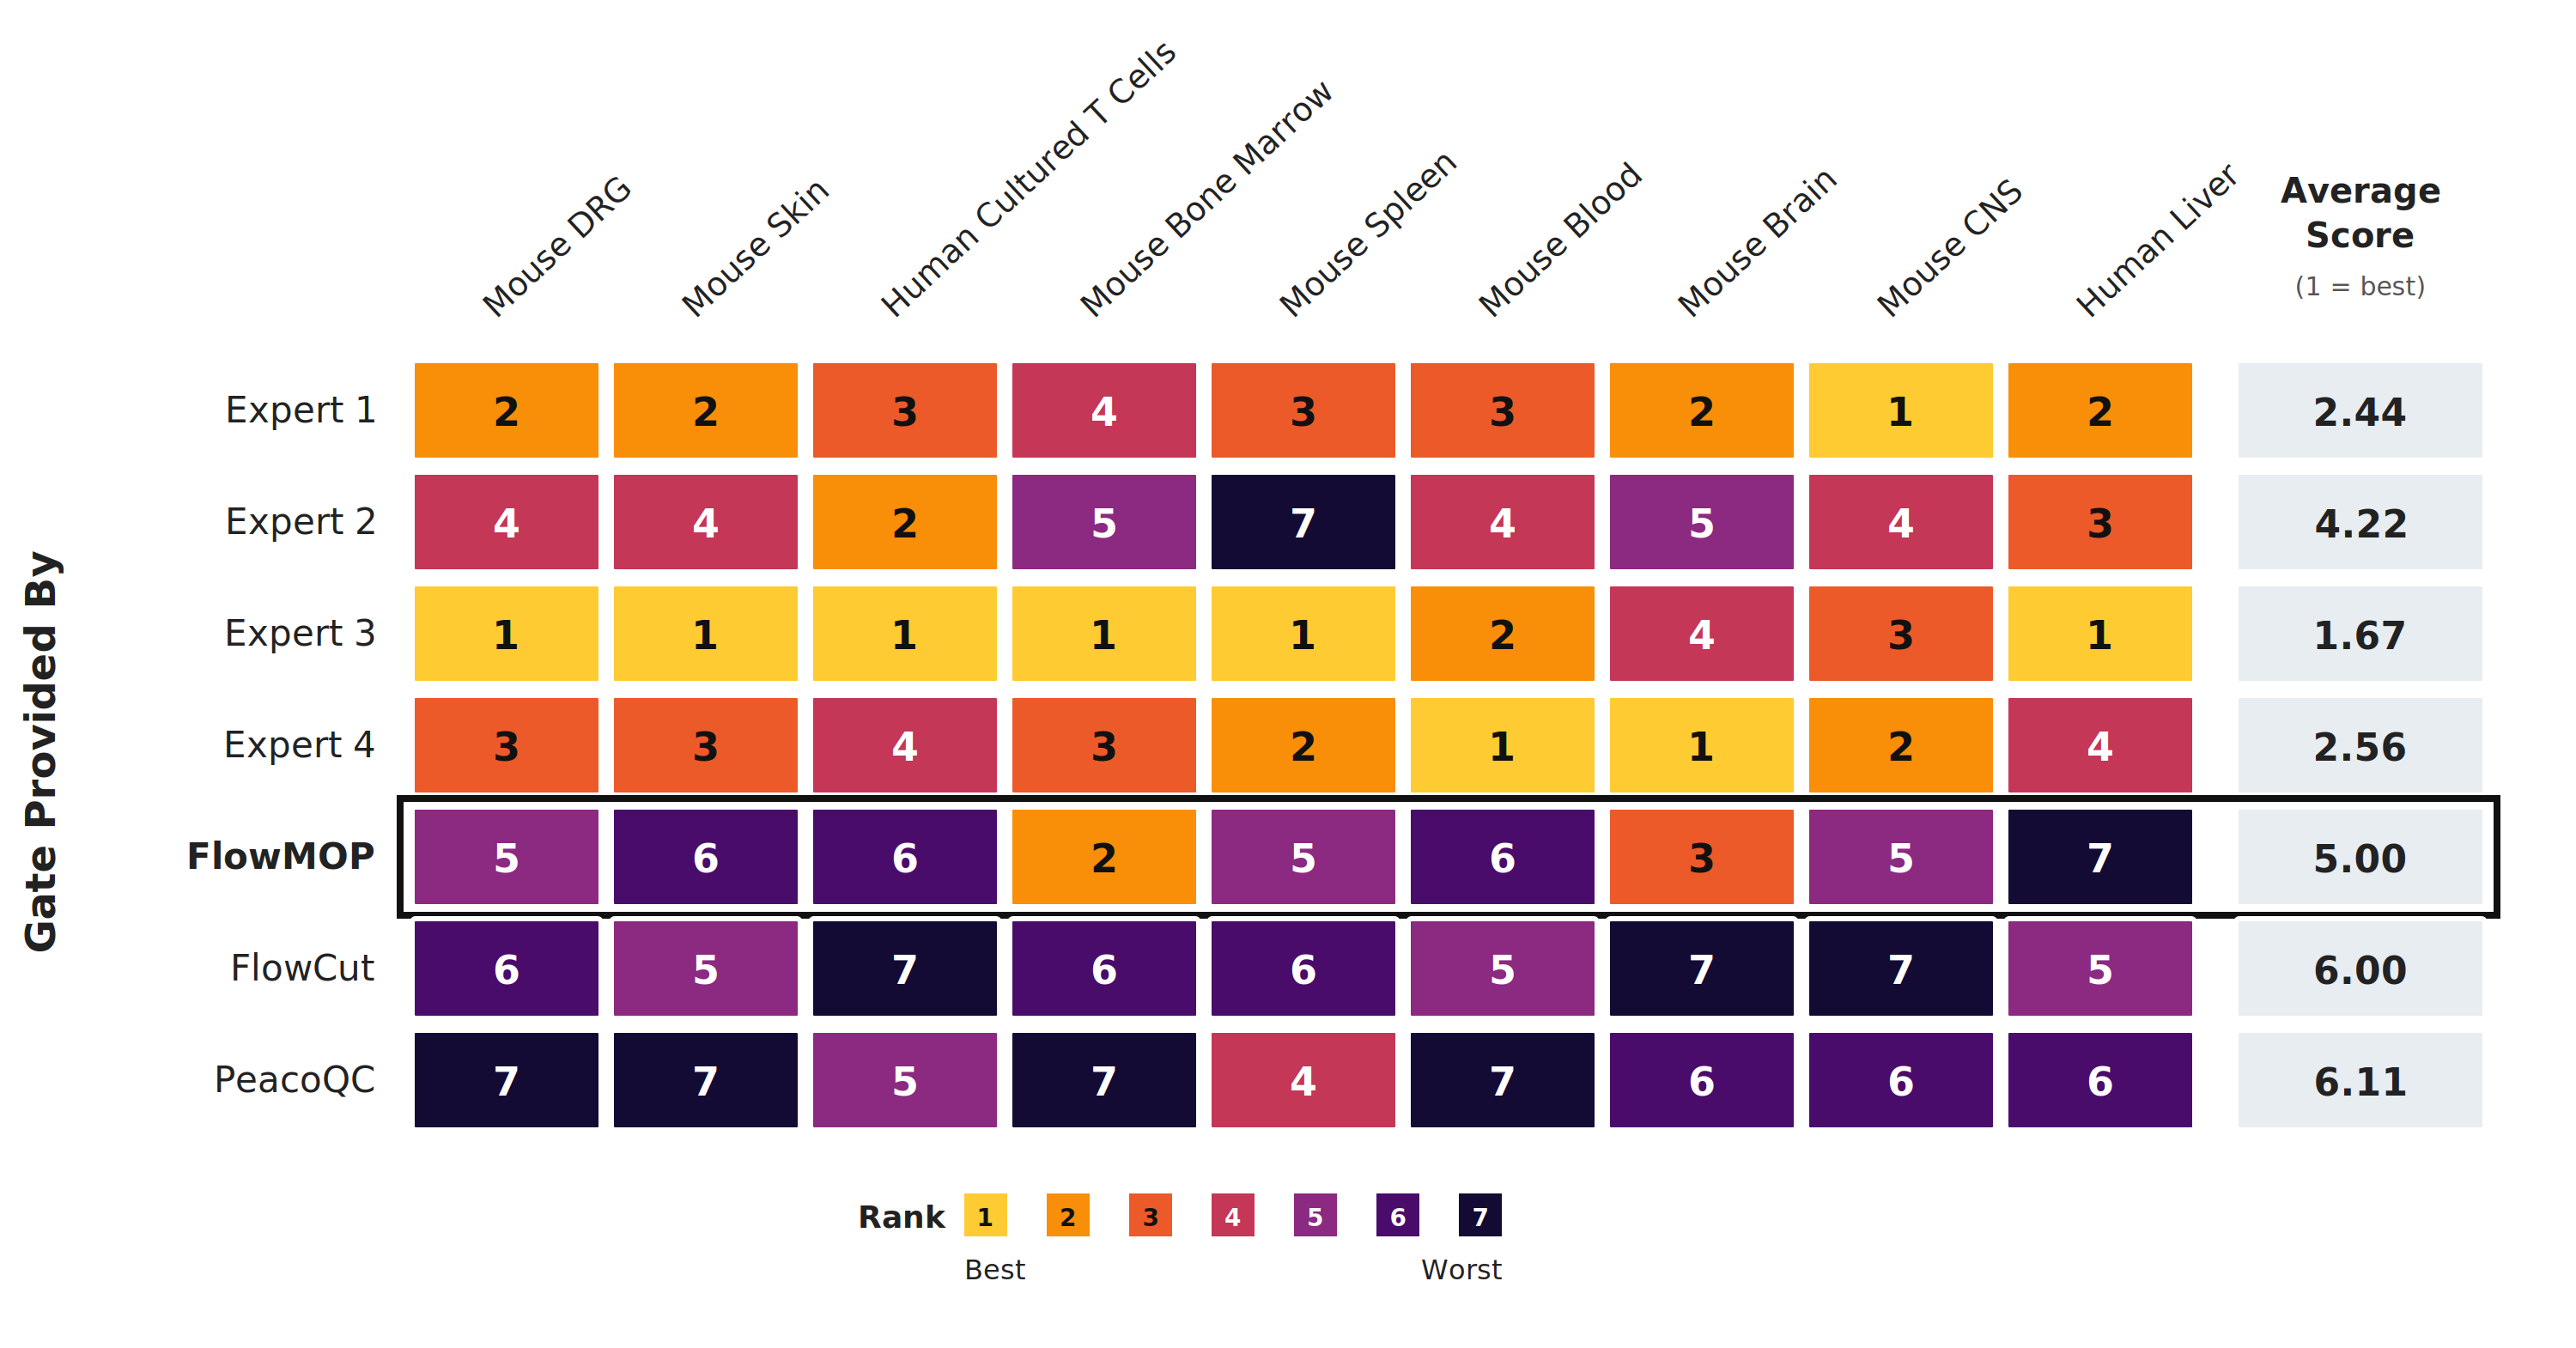
\includegraphics[width=\linewidth,height=0.82\textheight,keepaspectratio]{figs_data/Supp_fig_5.png}
\begingroup
\renewcommand{\thefigure}{S5}
\caption{Expert preference rankings for time gates provided by four human experts, FlowMOP (black border), FlowCut, and PeacoQC across nine datasets. Rows indicate the gate provider, and the final column shows the mean rank across datasets. Rank 1 indicates greatest preference; therefore, a lower average score indicates greater preference. Abbreviations: DRG, dorsal root ganglion; CNS, central nervous system.}
\endgroup
\end{figure}

In the biological datasets, FlowMOP had the lowest mean rank among the
algorithmic time-gating approaches (Fig. S5). In the mouse brain and
mouse bone marrow tasks, it ranked third and second, respectively (Fig.
S5). On a Bayesian analysis, FlowMOP was observed to be substantially
preferred to FlowCut (BF = 5.39, P = 84.3\%) and strongly preferred to
PeacoQC (BF = 12.10, P = 92.4\%). FlowMOP was ranked inferiorly to all
human experts with strong to decisive evidence (Expert 2 BF = 10.55, P =
91.3\%, all others BF \textgreater{} 100, P = 100\%).

\begin{figure}[p]
\centering
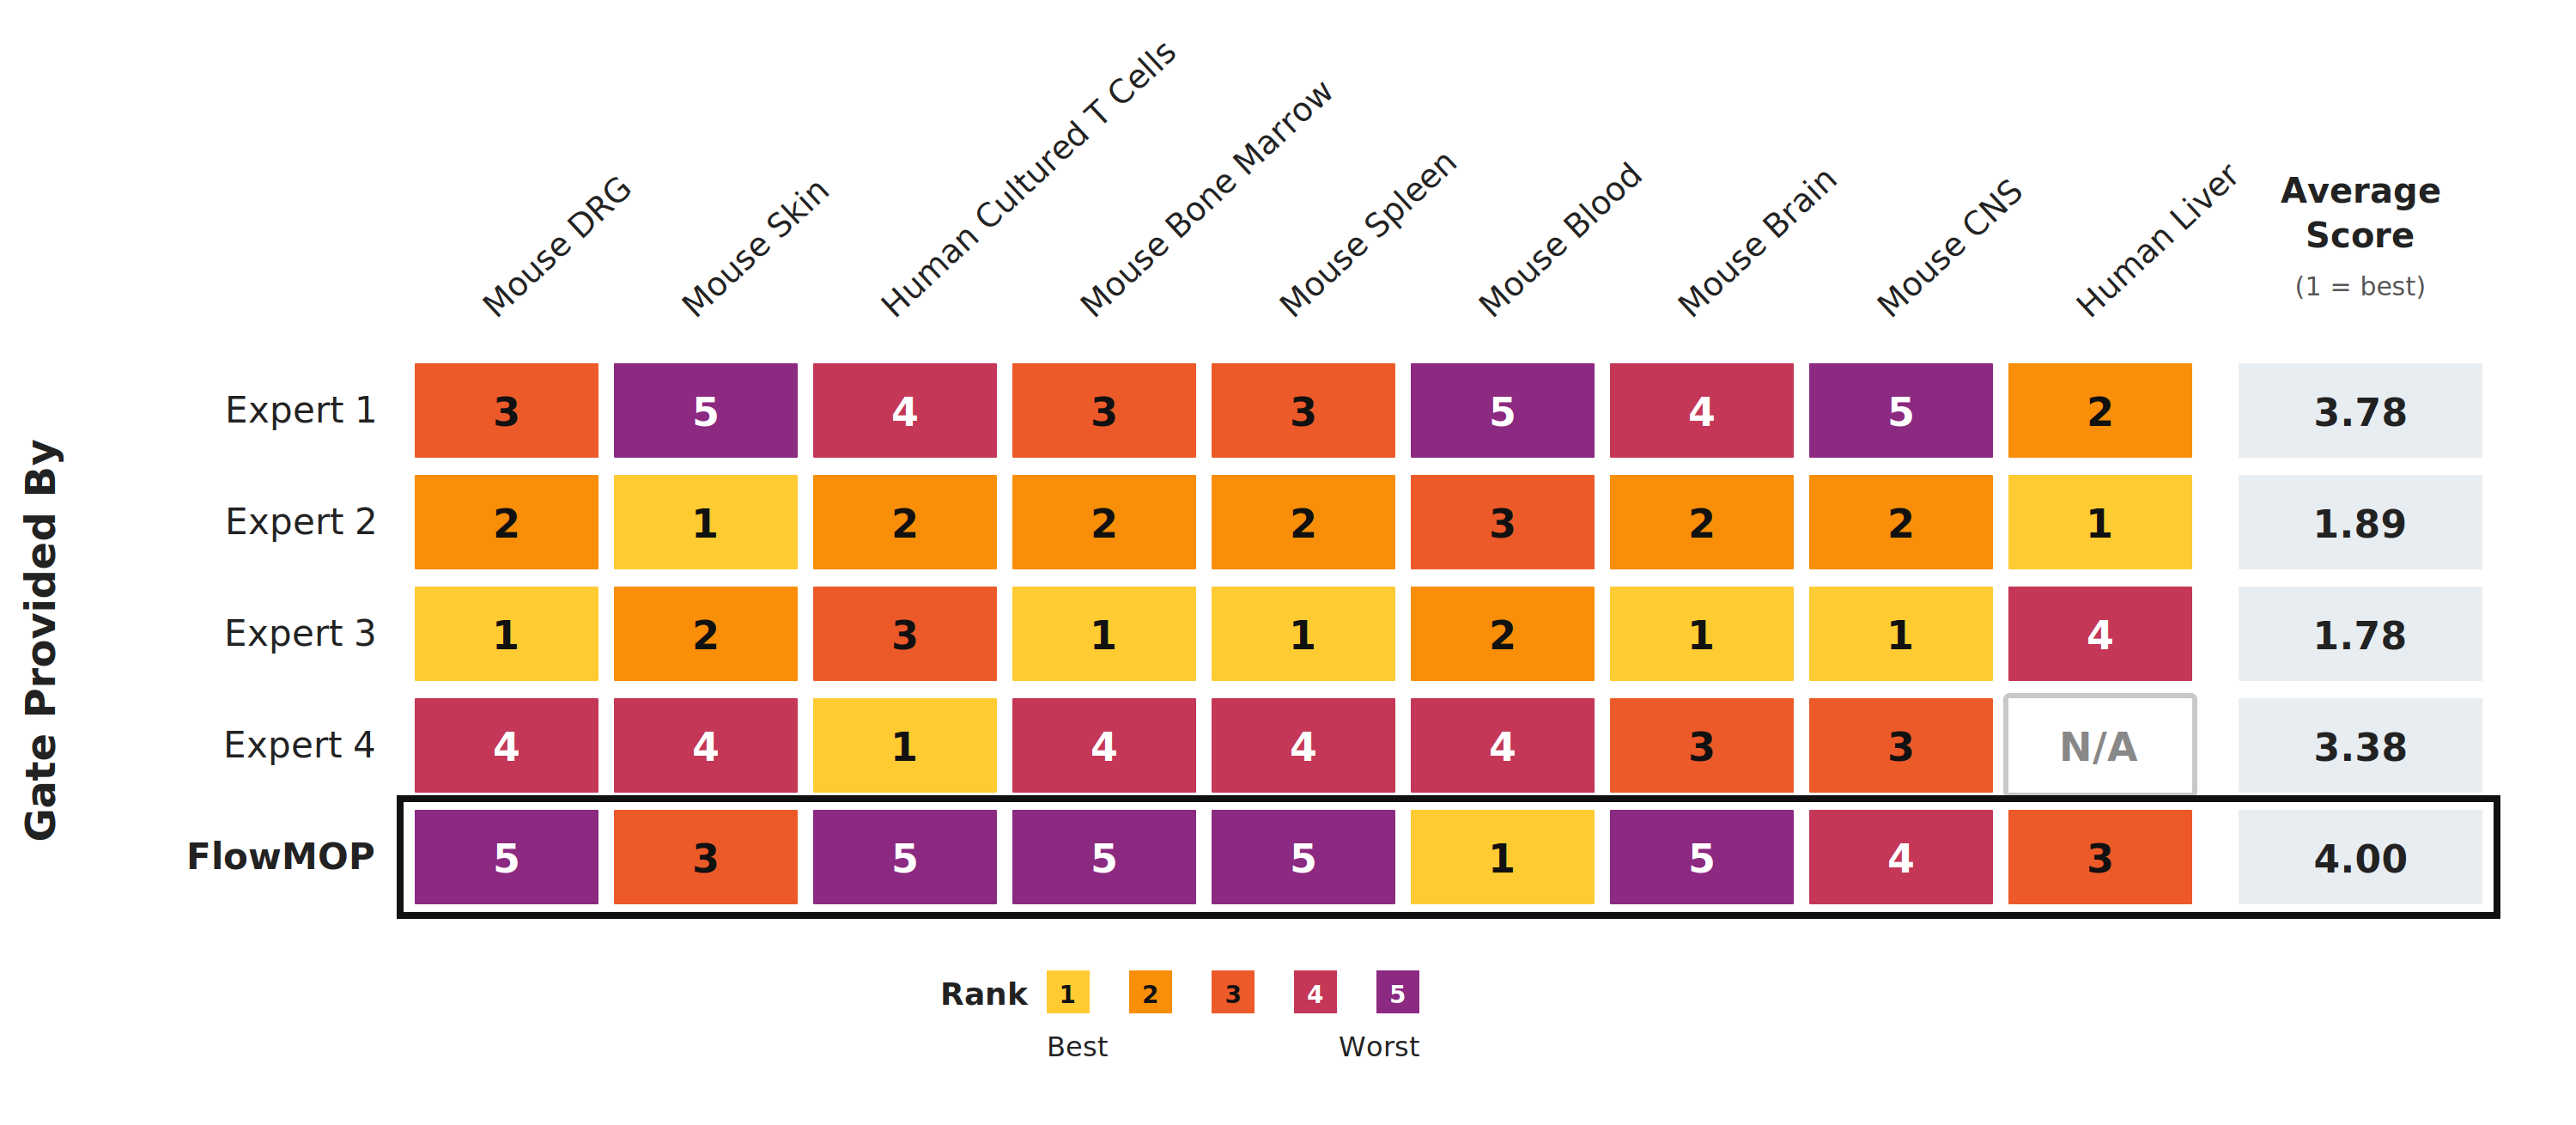
\includegraphics[width=\linewidth,height=0.82\textheight,keepaspectratio]{FlowMOP_submission_media/image6_revised.png}
\begingroup
\renewcommand{\thefigure}{S6}
\caption{Expert preference rankings for debris gates provided by four human experts and FlowMOP (black border) across nine datasets. Rows indicate the gate provider, and the final column shows the mean rank across available datasets. Rank 1 indicates greatest preference; therefore, a lower average score indicates greater preference. N/A denotes an unavailable gate.}
\endgroup
\end{figure}

\begin{figure}[p]
\centering
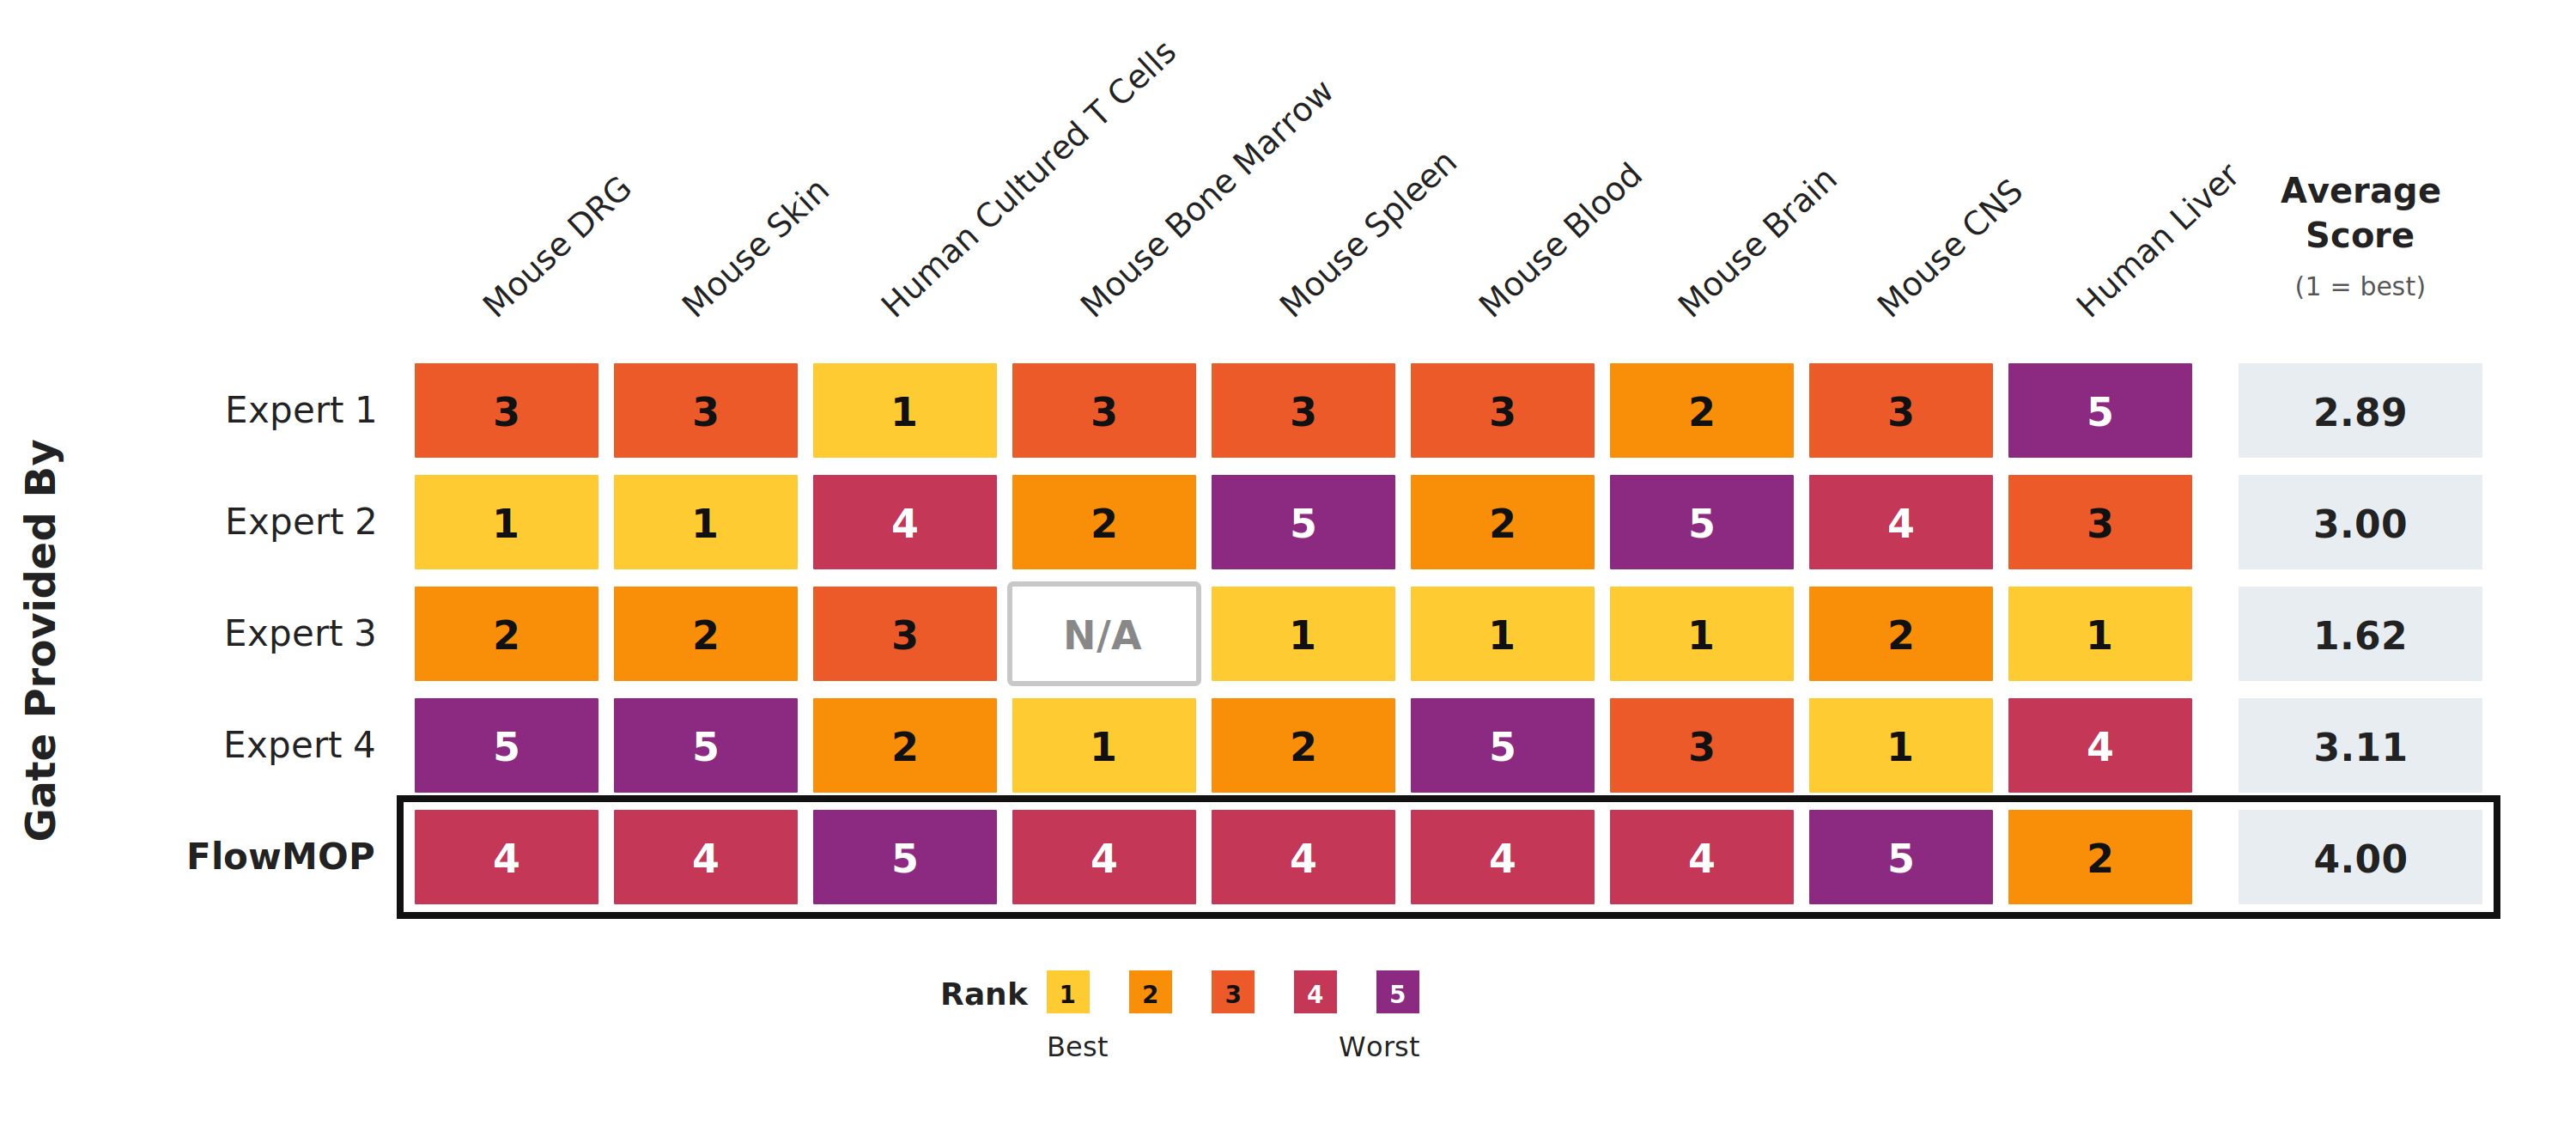
\includegraphics[width=\linewidth,height=0.82\textheight,keepaspectratio]{FlowMOP_submission_media/image7_revised.png}
\begingroup
\renewcommand{\thefigure}{S7}
\caption{Expert preference rankings for doublet gates provided by four human experts and FlowMOP (black border) across nine datasets. Rows indicate the gate provider, and the final column shows the mean rank across available datasets. Rank 1 indicates greatest preference; therefore, a lower average score indicates greater preference. N/A denotes an unavailable gate.}
\endgroup
\end{figure}

FlowMOP had the highest mean rank when compared with the human experts
for debris and doublet removal (Figs. S6, S7). On a Bayesian analysis,
substantial to strong evidence was observed for FlowMOP being inferior
to Expert 1 (BF = 5.87, P = 85.5\%), Expert 4 (BF = 12.85, P = 92.8\%),
and Experts 2 and 3 (BF \textgreater{} 100, P = 100\%) in debris
removal. In doublet removal, FlowMOP was weakly inferiorly ranked to
Expert 4 (BF = 3.14, P = 75.8\%), substantially inferiorly ranked to
Expert 1 (BF = 5.67, P = 85.0\%), strongly inferiorly ranked to Expert 2
(BF = 14.38, P = 93.5\%), and decisively inferiorly ranked to Expert 3
(BF \textgreater{} 100, P = 100\%).

FlowMOP's relative expert preference varied across datasets. For debris,
it ranked first in the mouse blood task and third in the human liver and
mouse skin datasets. In the doublet task, FlowMOP ranked second in the
human liver task. Complete dataset-level rankings and mean ranks are
shown in Figures S5-S7.

\begin{figure}[p]
\centering
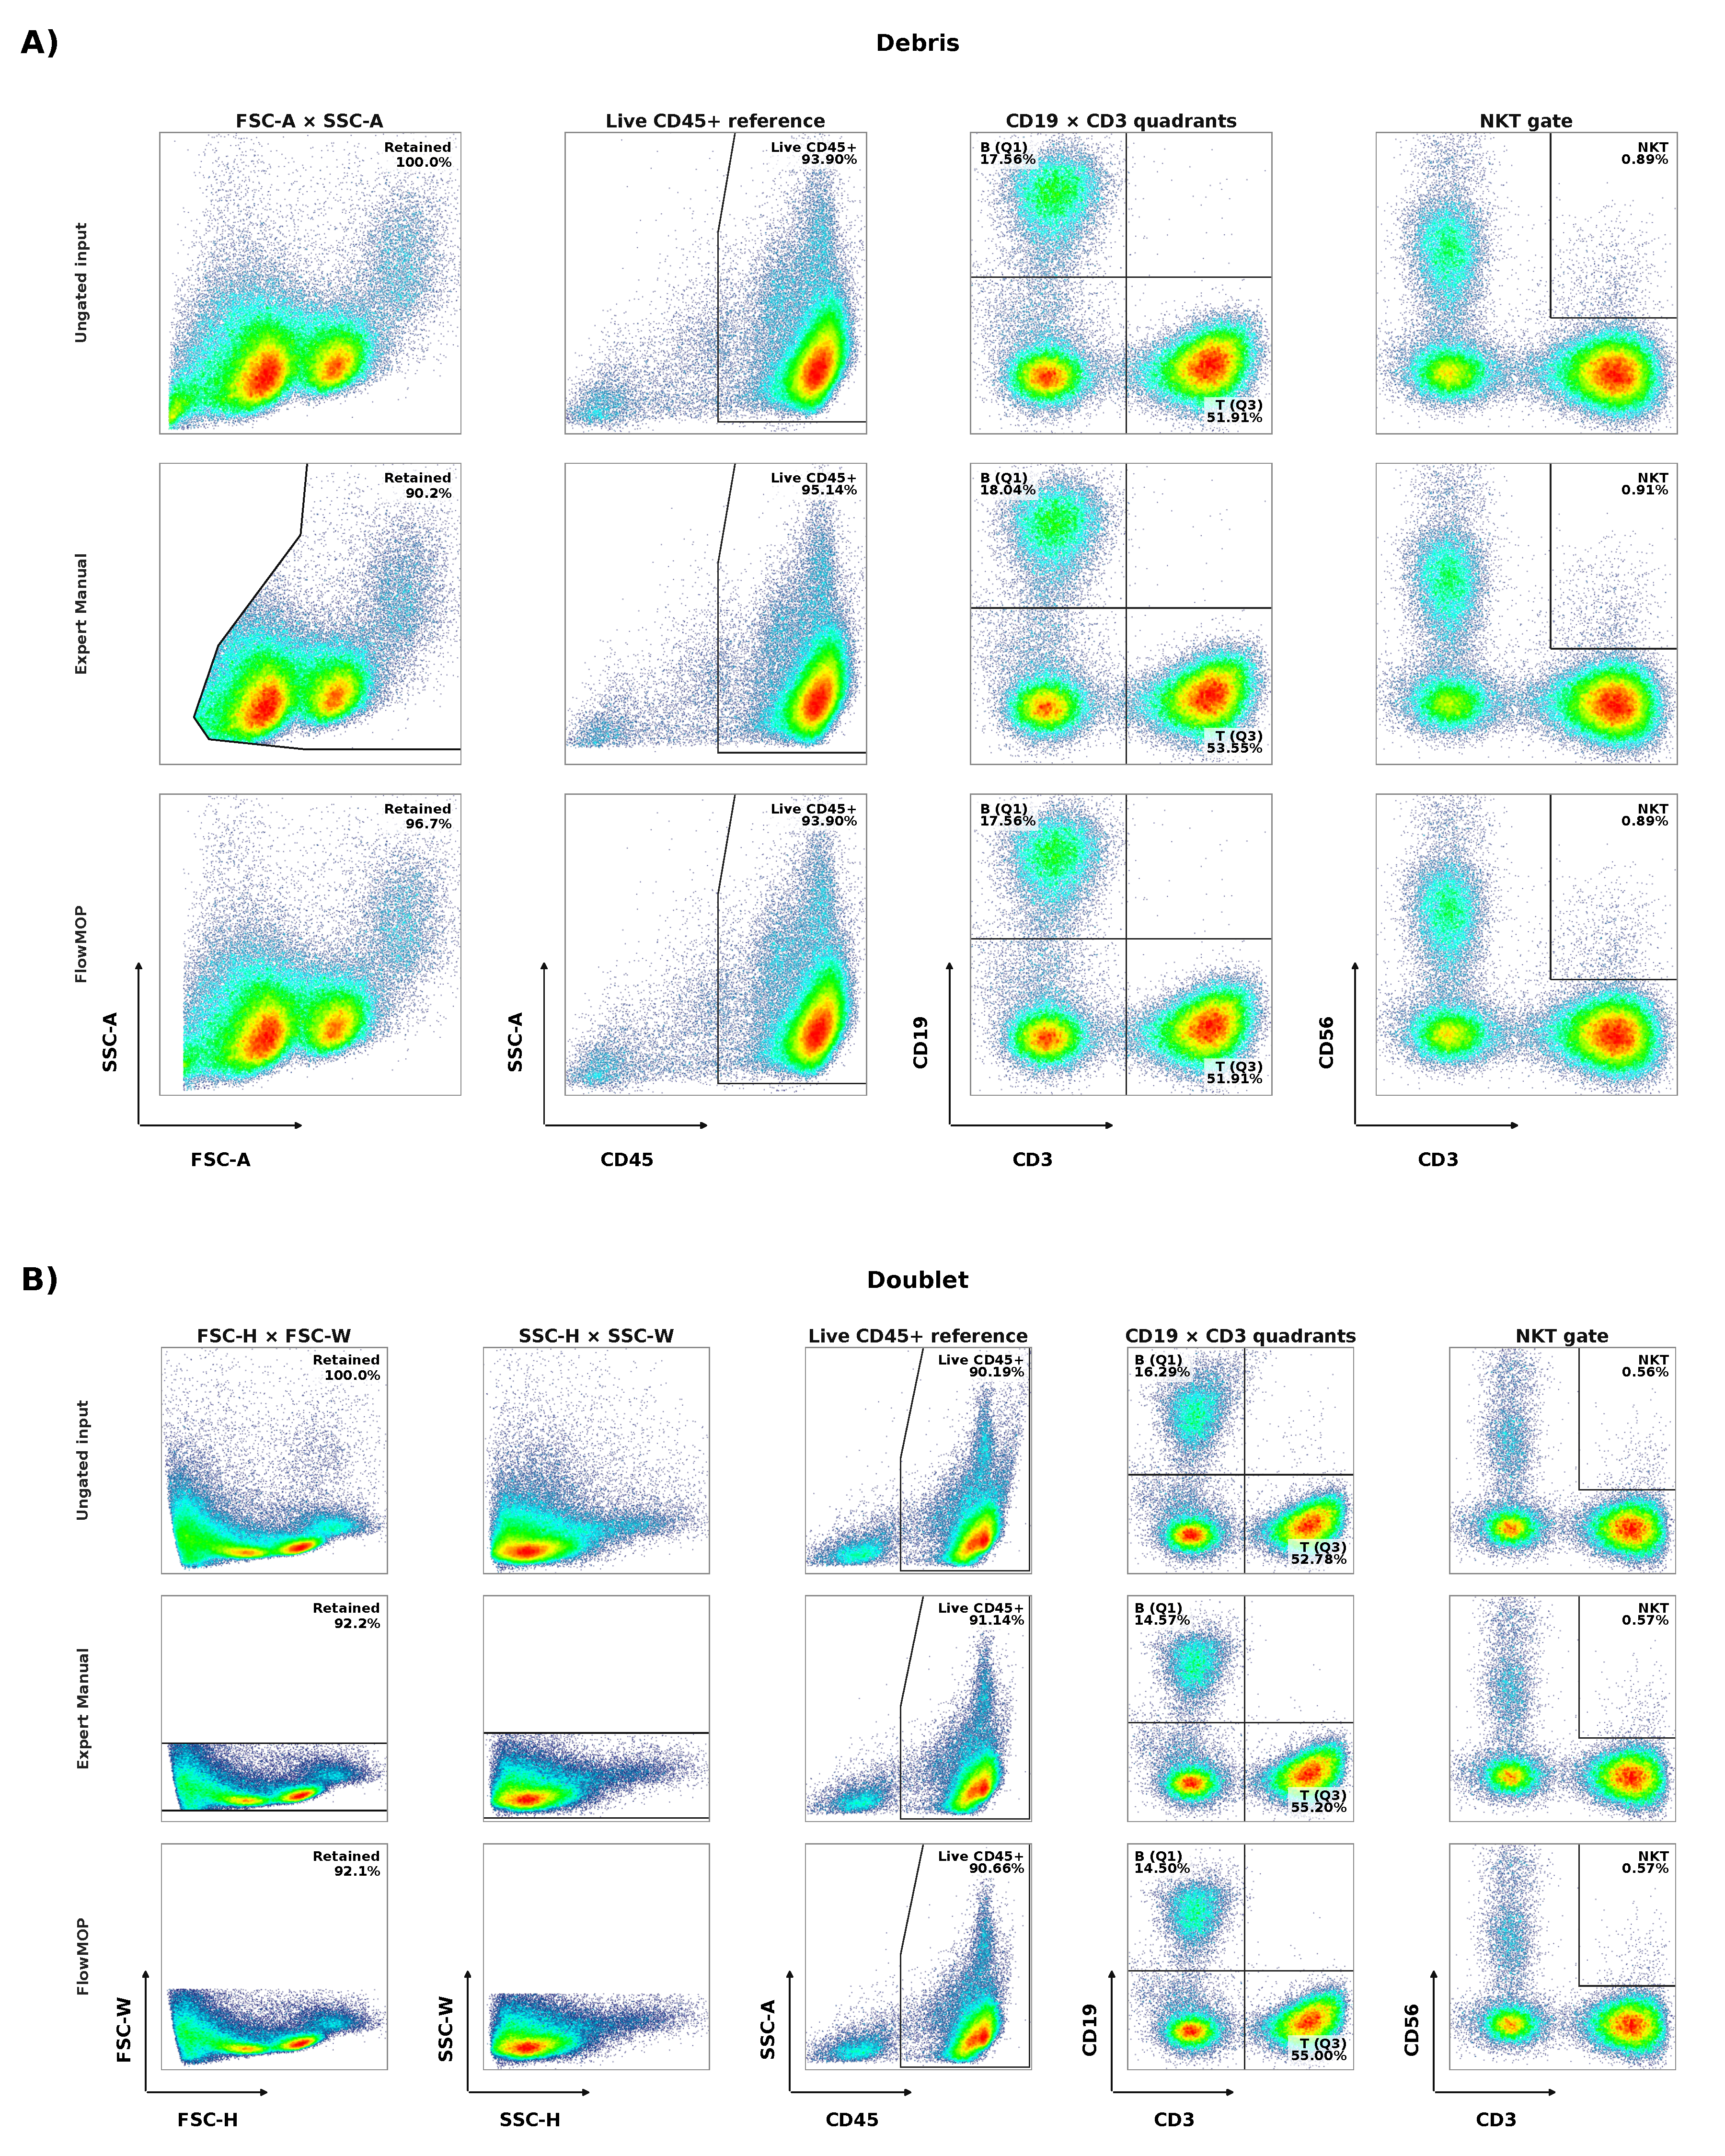
\includegraphics[width=\linewidth,height=0.68\textheight,keepaspectratio,trim=0pt 930pt 0pt 0pt,clip]{figs_data/Supp_fig_8.pdf}
\begingroup
\renewcommand{\thefigure}{S8}
\caption{Representative debris and doublet preprocessing projections. A) Debris comparison for Ungated input, Expert Manual, and FlowMOP. B) Doublet comparison for Ungated input, Expert Manual, and FlowMOP. Each row also shows the standalone Live CD45+ reference and the corresponding B/T and NKT gates evaluated without a CD45+ parent. The corresponding module-specific statistics are reported in Figure 6B,C.}
\endgroup
\end{figure}
\clearpage
\begin{figure}[p]
\centering
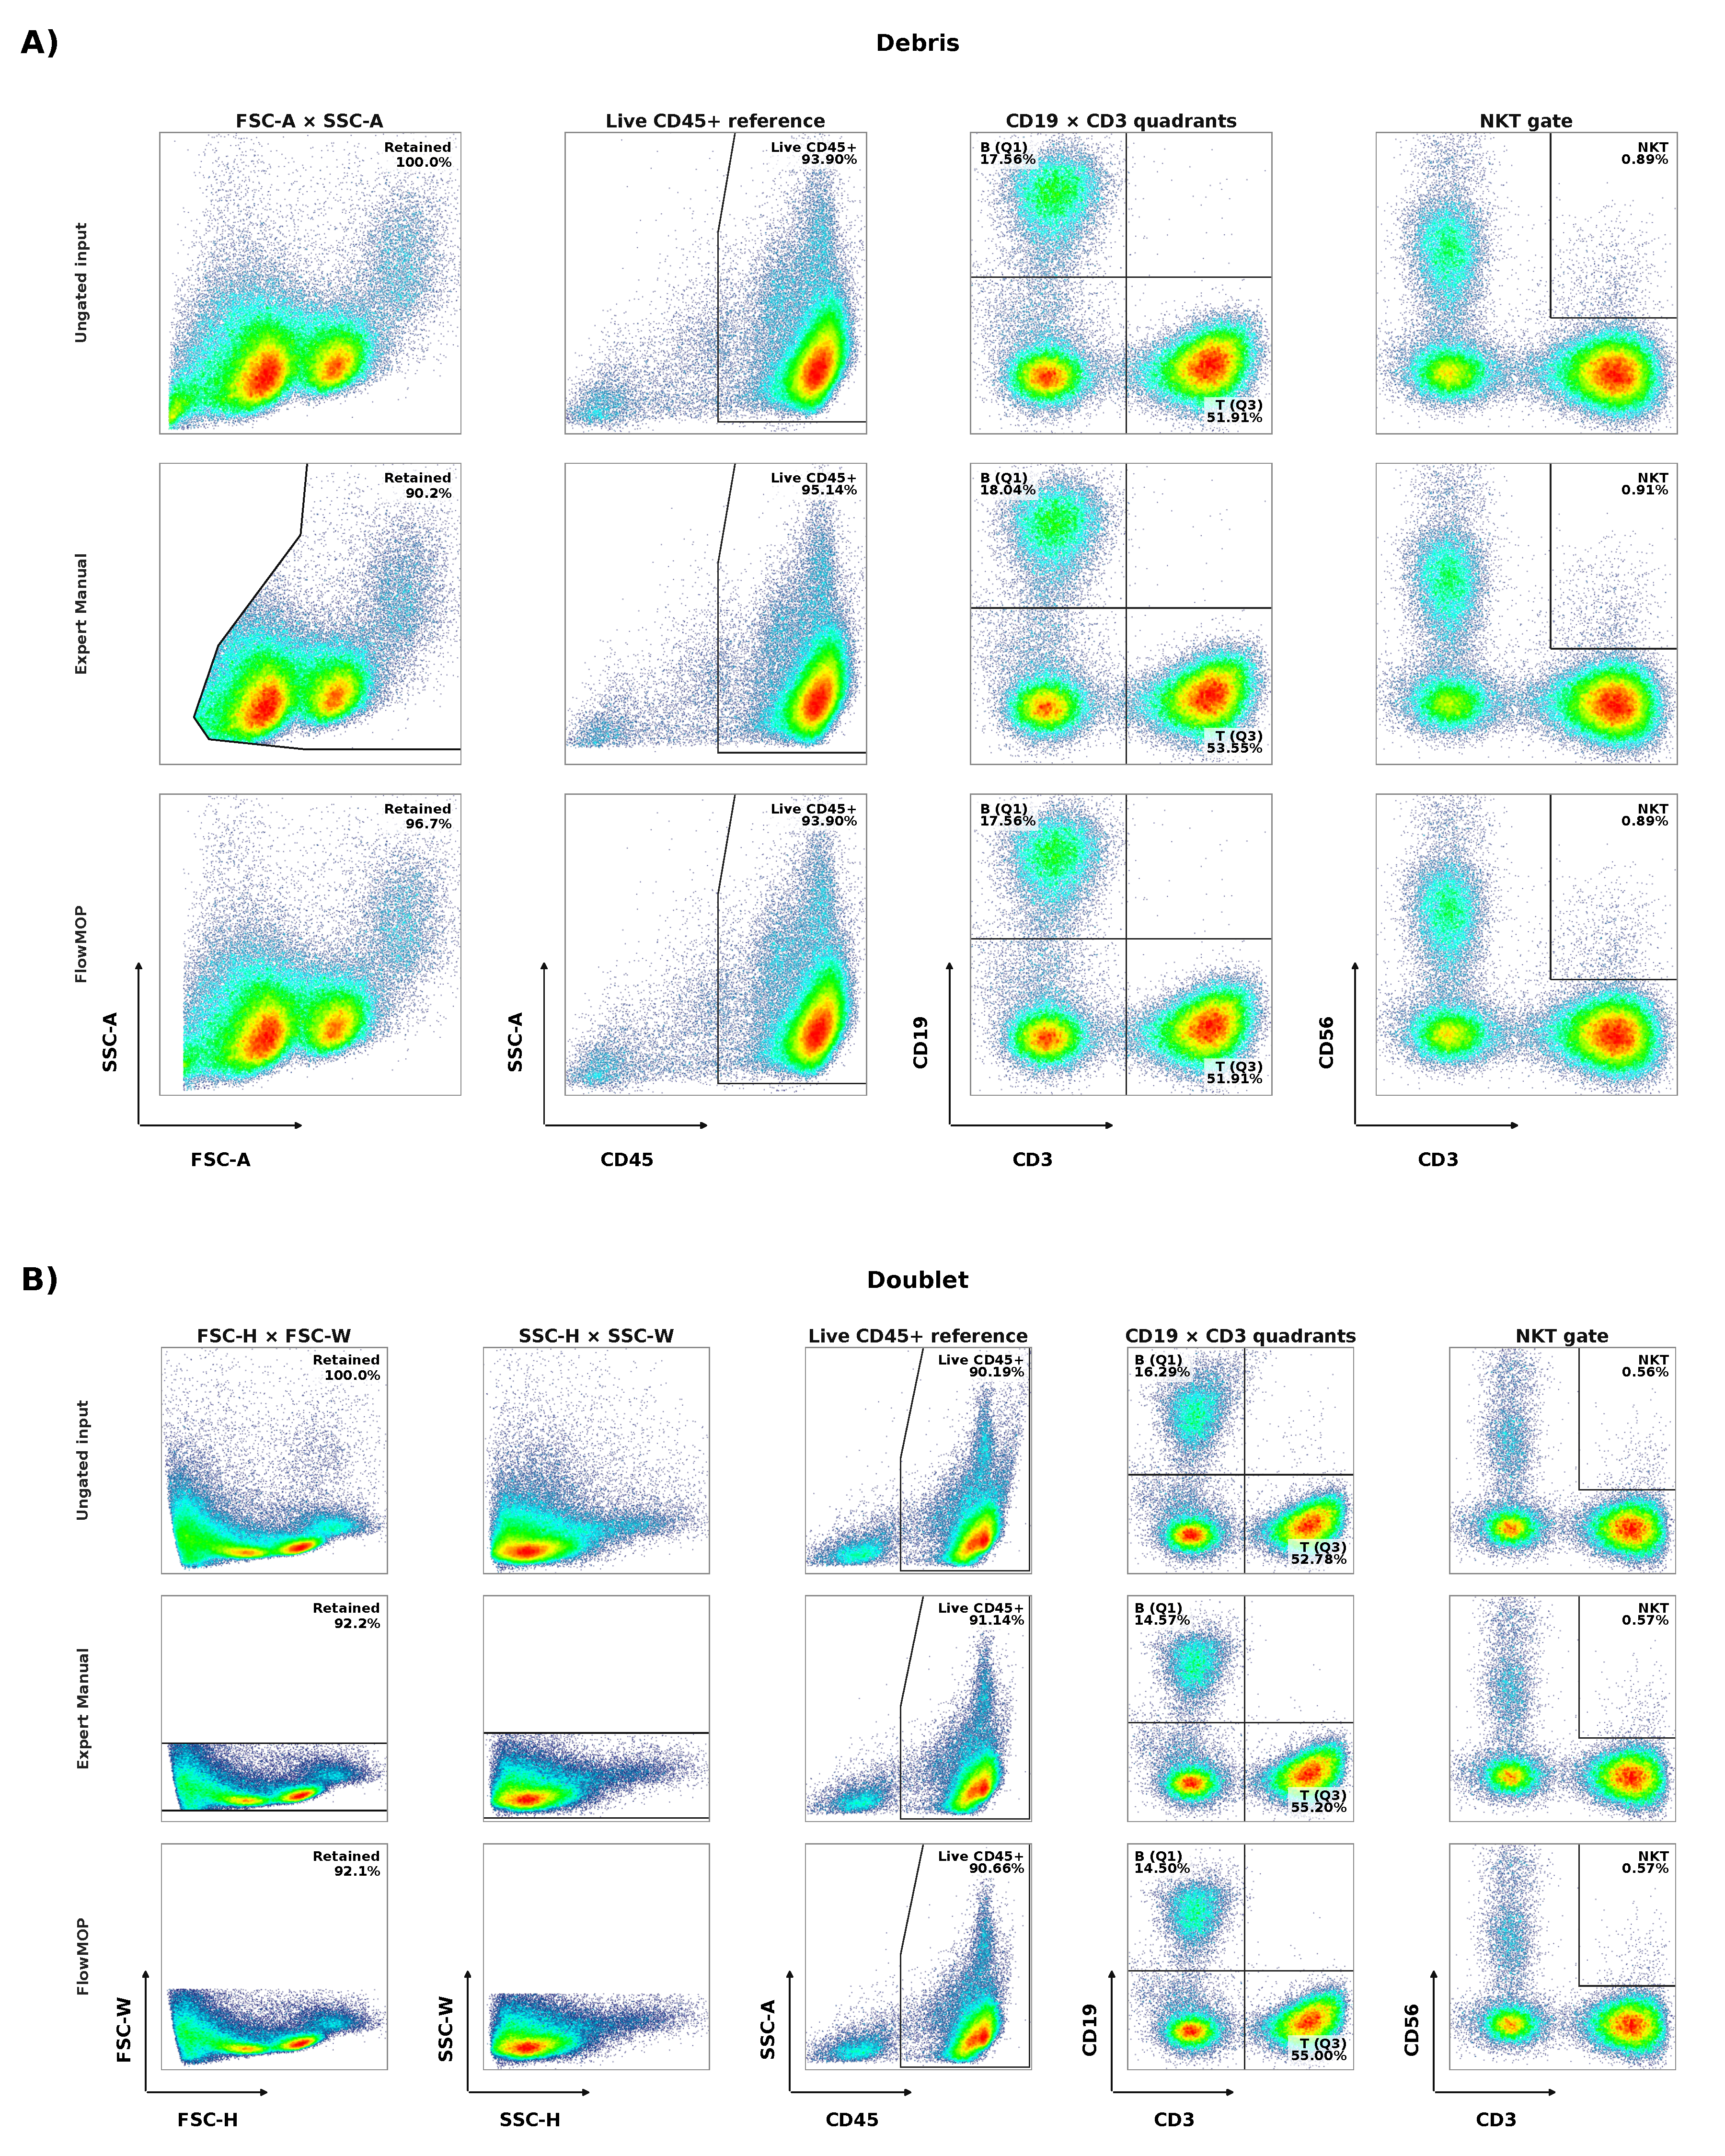
\includegraphics[width=\linewidth,height=0.58\textheight,keepaspectratio,trim=0pt 0pt 0pt 1240pt,clip]{figs_data/Supp_fig_8.pdf}
\begingroup
\renewcommand{\thefigure}{S8}
\caption*{\textbf{Figure S8 (continued)}}
\endgroup
\end{figure}
\clearpage

\FloatBarrier

\clearpage

\section{References}\label{references}

\begin{hangparas}{1.5em}{1}

{[}S1{]} Noah Castelo, Maarten W. Bos, and Donald R. Lehmann. 2019.
Task-Dependent Algorithm Aversion. Journal of Marketing Research 56, 5
(October 2019), 809--825. \url{https://doi.org/10.1177/0022243719851788}

\end{hangparas}

\end{document}
